% Options for packages loaded elsewhere
\PassOptionsToPackage{unicode}{hyperref}
\PassOptionsToPackage{hyphens}{url}
\documentclass[
  11pt,
]{article}
\usepackage{xcolor}
\usepackage[margin=1in]{geometry}
\usepackage{amsmath,amssymb}
\setcounter{secnumdepth}{-\maxdimen} % remove section numbering
\usepackage{iftex}
\ifPDFTeX
  \usepackage[T1]{fontenc}
  \usepackage[utf8]{inputenc}
  \usepackage{textcomp} % provide euro and other symbols
\else % if luatex or xetex
  \usepackage{unicode-math} % this also loads fontspec
  \defaultfontfeatures{Scale=MatchLowercase}
  \defaultfontfeatures[\rmfamily]{Ligatures=TeX,Scale=1}
\fi
\usepackage{lmodern}
\ifPDFTeX\else
  % xetex/luatex font selection
\fi
% Use upquote if available, for straight quotes in verbatim environments
\IfFileExists{upquote.sty}{\usepackage{upquote}}{}
\IfFileExists{microtype.sty}{% use microtype if available
  \usepackage[]{microtype}
  \UseMicrotypeSet[protrusion]{basicmath} % disable protrusion for tt fonts
}{}
\makeatletter
\@ifundefined{KOMAClassName}{% if non-KOMA class
  \IfFileExists{parskip.sty}{%
    \usepackage{parskip}
  }{% else
    \setlength{\parindent}{0pt}
    \setlength{\parskip}{6pt plus 2pt minus 1pt}}
}{% if KOMA class
  \KOMAoptions{parskip=half}}
\makeatother
\usepackage{color}
\usepackage{fancyvrb}
\newcommand{\VerbBar}{|}
\newcommand{\VERB}{\Verb[commandchars=\\\{\}]}
\DefineVerbatimEnvironment{Highlighting}{Verbatim}{commandchars=\\\{\}}
% Add ',fontsize=\small' for more characters per line
\newenvironment{Shaded}{}{}
\newcommand{\AlertTok}[1]{\textcolor[rgb]{1.00,0.00,0.00}{\textbf{#1}}}
\newcommand{\AnnotationTok}[1]{\textcolor[rgb]{0.38,0.63,0.69}{\textbf{\textit{#1}}}}
\newcommand{\AttributeTok}[1]{\textcolor[rgb]{0.49,0.56,0.16}{#1}}
\newcommand{\BaseNTok}[1]{\textcolor[rgb]{0.25,0.63,0.44}{#1}}
\newcommand{\BuiltInTok}[1]{\textcolor[rgb]{0.00,0.50,0.00}{#1}}
\newcommand{\CharTok}[1]{\textcolor[rgb]{0.25,0.44,0.63}{#1}}
\newcommand{\CommentTok}[1]{\textcolor[rgb]{0.38,0.63,0.69}{\textit{#1}}}
\newcommand{\CommentVarTok}[1]{\textcolor[rgb]{0.38,0.63,0.69}{\textbf{\textit{#1}}}}
\newcommand{\ConstantTok}[1]{\textcolor[rgb]{0.53,0.00,0.00}{#1}}
\newcommand{\ControlFlowTok}[1]{\textcolor[rgb]{0.00,0.44,0.13}{\textbf{#1}}}
\newcommand{\DataTypeTok}[1]{\textcolor[rgb]{0.56,0.13,0.00}{#1}}
\newcommand{\DecValTok}[1]{\textcolor[rgb]{0.25,0.63,0.44}{#1}}
\newcommand{\DocumentationTok}[1]{\textcolor[rgb]{0.73,0.13,0.13}{\textit{#1}}}
\newcommand{\ErrorTok}[1]{\textcolor[rgb]{1.00,0.00,0.00}{\textbf{#1}}}
\newcommand{\ExtensionTok}[1]{#1}
\newcommand{\FloatTok}[1]{\textcolor[rgb]{0.25,0.63,0.44}{#1}}
\newcommand{\FunctionTok}[1]{\textcolor[rgb]{0.02,0.16,0.49}{#1}}
\newcommand{\ImportTok}[1]{\textcolor[rgb]{0.00,0.50,0.00}{\textbf{#1}}}
\newcommand{\InformationTok}[1]{\textcolor[rgb]{0.38,0.63,0.69}{\textbf{\textit{#1}}}}
\newcommand{\KeywordTok}[1]{\textcolor[rgb]{0.00,0.44,0.13}{\textbf{#1}}}
\newcommand{\NormalTok}[1]{#1}
\newcommand{\OperatorTok}[1]{\textcolor[rgb]{0.40,0.40,0.40}{#1}}
\newcommand{\OtherTok}[1]{\textcolor[rgb]{0.00,0.44,0.13}{#1}}
\newcommand{\PreprocessorTok}[1]{\textcolor[rgb]{0.74,0.48,0.00}{#1}}
\newcommand{\RegionMarkerTok}[1]{#1}
\newcommand{\SpecialCharTok}[1]{\textcolor[rgb]{0.25,0.44,0.63}{#1}}
\newcommand{\SpecialStringTok}[1]{\textcolor[rgb]{0.73,0.40,0.53}{#1}}
\newcommand{\StringTok}[1]{\textcolor[rgb]{0.25,0.44,0.63}{#1}}
\newcommand{\VariableTok}[1]{\textcolor[rgb]{0.10,0.09,0.49}{#1}}
\newcommand{\VerbatimStringTok}[1]{\textcolor[rgb]{0.25,0.44,0.63}{#1}}
\newcommand{\WarningTok}[1]{\textcolor[rgb]{0.38,0.63,0.69}{\textbf{\textit{#1}}}}
\usepackage{graphicx}
\makeatletter
\newsavebox\pandoc@box
\newcommand*\pandocbounded[1]{% scales image to fit in text height/width
  \sbox\pandoc@box{#1}%
  \Gscale@div\@tempa{\textheight}{\dimexpr\ht\pandoc@box+\dp\pandoc@box\relax}%
  \Gscale@div\@tempb{\linewidth}{\wd\pandoc@box}%
  \ifdim\@tempb\p@<\@tempa\p@\let\@tempa\@tempb\fi% select the smaller of both
  \ifdim\@tempa\p@<\p@\scalebox{\@tempa}{\usebox\pandoc@box}%
  \else\usebox{\pandoc@box}%
  \fi%
}
% Set default figure placement to htbp
\def\fps@figure{htbp}
\makeatother
\setlength{\emergencystretch}{3em} % prevent overfull lines
\providecommand{\tightlist}{%
  \setlength{\itemsep}{0pt}\setlength{\parskip}{0pt}}
\usepackage{amsmath}
\usepackage{amssymb}
\usepackage{unicode-math}
\usepackage{graphicx}
\usepackage{bookmark}
\IfFileExists{xurl.sty}{\usepackage{xurl}}{} % add URL line breaks if available
\urlstyle{same}
\hypersetup{
  pdftitle={Numerical Demonstration of the Heisenberg Uncertainty Principle using Gaussian Wave Packets},
  pdfauthor={Stefan Len},
  hidelinks,
  pdfcreator={LaTeX via pandoc}}

\title{Numerical Demonstration of the Heisenberg Uncertainty Principle
using Gaussian Wave Packets}
\author{Stefan Len}
\date{October 15, 2025}

\begin{document}
\maketitle

\section{Numerical Demonstration of the Heisenberg Uncertainty Principle
using Gaussian Wave
Packets}\label{numerical-demonstration-of-the-heisenberg-uncertainty-principle-using-gaussian-wave-packets}

\textbf{Stefan Len}

\emph{Independent Researcher}

\textbf{Date:} October 15, 2025

\begin{center}\rule{0.5\linewidth}{0.5pt}\end{center}

\subsection{Abstract}\label{abstract}

We present a minimal numerical demonstration of the Heisenberg
Uncertainty Principle using Gaussian wave packets in one spatial
dimension. By systematically varying the initial position spread, we
numerically verify the reciprocal relationship between position and
momentum uncertainties and confirm that their product remains bounded by
the theoretical minimum of ℏ/2. In addition, we simulate the free time
evolution of the wave packet, illustrating the spreading of the position
uncertainty while the momentum distribution remains constant. The
results highlight the role of Gaussian wave packets as
minimum-uncertainty states and provide an accessible, reproducible
teaching tool for quantum mechanics.

\textbf{Keywords:} Heisenberg uncertainty principle, Gaussian wave
packet, quantum mechanics, minimum uncertainty state, numerical
simulation, pedagogical tool

\begin{center}\rule{0.5\linewidth}{0.5pt}\end{center}

\subsection{1. Introduction}\label{introduction}

\subsubsection{1.1 The Heisenberg Uncertainty
Principle}\label{the-heisenberg-uncertainty-principle}

The Heisenberg Uncertainty Principle, formulated by Werner Heisenberg in
1927 {[}1{]}, represents one of the most fundamental departures of
quantum mechanics from classical physics. It establishes that certain
pairs of physical quantities---canonical conjugates such as position and
momentum---cannot be simultaneously measured with arbitrary precision.
Mathematically, for position x and momentum p:

\[\Delta x \cdot \Delta p \geq \frac{\hbar}{2}\]

where Δx and Δp are the standard deviations (uncertainties) of position
and momentum, respectively, and ℏ is the reduced Planck constant. This
inequality is not a statement about experimental limitations or
measurement disturbance, but rather reflects a fundamental property
inherent in the mathematical structure of quantum mechanics itself.

\subsubsection{1.2 Gaussian Wave Packets as Optimal
States}\label{gaussian-wave-packets-as-optimal-states}

Among all possible quantum states, Gaussian wave packets occupy a
privileged position: they saturate the uncertainty bound, achieving
equality in the Heisenberg relation {[}2{]}. For a Gaussian state:

\[\Delta x \cdot \Delta p = \frac{\hbar}{2}\]

This property designates Gaussian wave packets as minimum-uncertainty
states or coherent states, representing the closest quantum analog to
classical particles. Their dual nature---exhibiting optimal localization
in both position and momentum space simultaneously---makes them ideal
subjects for both theoretical analysis and pedagogical demonstration.

\subsubsection{1.3 Computational Approach and
Objectives}\label{computational-approach-and-objectives}

Numerical simulations provide direct, visual validation of abstract
quantum mechanical principles that often resist intuitive understanding.
This work employs a straightforward computational framework based on
Fast Fourier Transform (FFT) techniques to:

\begin{enumerate}
\def\labelenumi{\arabic{enumi}.}
\tightlist
\item
  Construct Gaussian wave packets with systematically varied position
  spreads
\item
  Compute momentum distributions via discrete Fourier transformation
\item
  Quantify position and momentum uncertainties numerically
\item
  Verify the Heisenberg uncertainty relation across parameter space
\item
  Simulate free time evolution to demonstrate wave packet spreading
\end{enumerate}

The primary objectives are to provide quantitative numerical
verification of the uncertainty principle, to illustrate the reciprocal
relationship between conjugate uncertainties, and to offer a
reproducible computational tool suitable for educational purposes in
quantum mechanics courses.

\begin{center}\rule{0.5\linewidth}{0.5pt}\end{center}

\subsection{2. Theory and Method}\label{theory-and-method}

\subsubsection{2.1 Quantum Mechanical
Framework}\label{quantum-mechanical-framework}

\paragraph{2.1.1 Wave Function and Probability
Interpretation}\label{wave-function-and-probability-interpretation}

In one-dimensional quantum mechanics, the state of a particle is
described by a complex-valued wave function ψ(x,t) satisfying the
Schrödinger equation. The probability density for finding the particle
at position x is:

\[\rho(x) = |\psi(x)|^2\]

normalized such that:

\[\int_{-\infty}^{\infty} |\psi(x)|^2 dx = 1\]

\paragraph{2.1.2 Position-Momentum
Duality}\label{position-momentum-duality}

The momentum-space representation is obtained through the Fourier
transform:

\[\Psi(p) = \frac{1}{\sqrt{2\pi\hbar}}\int_{-\infty}^{\infty} \psi(x)e^{-ipx/\hbar}dx\]

with corresponding probability density in momentum space:

\[\rho_p(p) = |\Psi(p)|^2\]

This dual representation---position and momentum as complementary
descriptions---lies at the heart of the uncertainty principle.

\subsubsection{2.2 Gaussian Wave Packet
Construction}\label{gaussian-wave-packet-construction}

\paragraph{2.2.1 Initial State}\label{initial-state}

A Gaussian wave packet centered at position x₀ with mean momentum p₀ has
the analytical form:

\[\psi(x,0) = \left(\frac{1}{2\pi\sigma_x^2}\right)^{1/4} \exp\left[-\frac{(x-x_0)^2}{4\sigma_x^2} + \frac{ip_0(x-x_0)}{\hbar}\right]\]

where σₓ is the initial position spread. For our simulations, we set x₀
= 0 and p₀ = 0 (particle at rest at the origin):

\[\psi(x,0) = \left(\frac{1}{2\pi\sigma_x^2}\right)^{1/4} \exp\left[-\frac{x^2}{4\sigma_x^2}\right]\]

\paragraph{2.2.2 Momentum Distribution}\label{momentum-distribution}

The Fourier transform of the initial Gaussian yields the momentum
distribution:

\[\Psi(p,0) = \left(\frac{2\sigma_x^2}{\pi\hbar^2}\right)^{1/4} \exp\left[-\frac{\sigma_x^2 p^2}{\hbar^2}\right]\]

This is also Gaussian, with spread:

\[\sigma_p = \frac{\hbar}{2\sigma_x}\]

demonstrating the reciprocal relationship: as σₓ increases, σₚ decreases
proportionally.

\subsubsection{2.3 Uncertainty
Quantification}\label{uncertainty-quantification}

\paragraph{2.3.1 Position Uncertainty}\label{position-uncertainty}

The position uncertainty is defined as the standard deviation:

\[\Delta x = \sqrt{\langle x^2 \rangle - \langle x \rangle^2}\]

where expectation values are computed as:

\[\langle x \rangle = \int_{-\infty}^{\infty} x|\psi(x)|^2 dx\]

\[\langle x^2 \rangle = \int_{-\infty}^{\infty} x^2|\psi(x)|^2 dx\]

For a Gaussian wave packet, Δx = σₓ exactly.

\paragraph{2.3.2 Momentum Uncertainty}\label{momentum-uncertainty}

Similarly, the momentum uncertainty is:

\[\Delta p = \sqrt{\langle p^2 \rangle - \langle p \rangle^2}\]

with:

\[\langle p \rangle = \int_{-\infty}^{\infty} p|\Psi(p)|^2 dp\]

\[\langle p^2 \rangle = \int_{-\infty}^{\infty} p^2|\Psi(p)|^2 dp\]

For the Gaussian momentum distribution, Δp = ℏ/(2σₓ).

\paragraph{2.3.3 Uncertainty Product}\label{uncertainty-product}

Combining these results:

\[\Delta x \cdot \Delta p = \sigma_x \cdot \frac{\hbar}{2\sigma_x} = \frac{\hbar}{2}\]

This confirms analytically that Gaussian wave packets achieve the
minimum uncertainty bound.

\subsubsection{2.4 Time Evolution}\label{time-evolution}

\paragraph{2.4.1 Free Particle Dynamics}\label{free-particle-dynamics}

For a free particle (no external potential), the time-evolved wave
function can be obtained exactly. The position uncertainty evolves as:

\[\sigma_x(t) = \sigma_x(0)\sqrt{1 + \left(\frac{\hbar t}{2m\sigma_x^2(0)}\right)^2}\]

where m is the particle mass. This demonstrates that position
uncertainty grows monotonically with time---a phenomenon known as wave
packet spreading.

\paragraph{2.4.2 Momentum Conservation}\label{momentum-conservation}

Crucially, the momentum distribution remains unchanged during free
evolution:

\[\Psi(p,t) = \Psi(p,0)\]

Therefore:

\[\Delta p(t) = \Delta p(0) = \text{constant}\]

The uncertainty product thus evolves as:

\[\Delta x(t) \cdot \Delta p = \sigma_x(t) \cdot \frac{\hbar}{2\sigma_x(0)} \geq \frac{\hbar}{2}\]

increasing with time but always satisfying the uncertainty relation.

\subsubsection{2.5 Numerical
Implementation}\label{numerical-implementation}

\paragraph{2.5.1 Spatial Discretization}\label{spatial-discretization}

We discretize position space on a uniform grid with N = 16384 points:

\[x_j = -\frac{L}{2} + j\Delta x, \quad j = 0,1,\ldots,N-1\]

where L = 200 is the spatial domain size and Δx = L/N is the grid
spacing. The wave function is sampled at these points: ψⱼ = ψ(xⱼ).

\paragraph{2.5.2 Fourier Transform}\label{fourier-transform}

The momentum distribution is computed using the Fast Fourier Transform
(FFT):

\[\Psi_k = \text{FFT}[\psi_j] \cdot \frac{\Delta x}{\sqrt{2\pi\hbar}}\]

with corresponding momentum grid:

\[p_k = \hbar k_k, \quad k_k = \frac{2\pi}{L}\left(k - \frac{N}{2}\right)\]

for k = 0, 1, \ldots, N-1.

\paragraph{2.5.3 Expectation Value
Calculation}\label{expectation-value-calculation}

Position expectation values are computed numerically using trapezoidal
integration:

\[\langle x \rangle \approx \sum_{j=0}^{N-1} x_j |\psi_j|^2 \Delta x\]

\[\langle x^2 \rangle \approx \sum_{j=0}^{N-1} x_j^2 |\psi_j|^2 \Delta x\]

Similarly for momentum:

\[\langle p \rangle \approx \sum_{k=0}^{N-1} p_k |\Psi_k|^2 \Delta p\]

\[\langle p^2 \rangle \approx \sum_{k=0}^{N-1} p_k^2 |\Psi_k|^2 \Delta p\]

where Δp = 2πℏ/L is the momentum grid spacing.

\paragraph{2.5.4 Time Evolution
Algorithm}\label{time-evolution-algorithm}

Free time evolution is implemented using the split-operator method. The
kinetic energy operator in momentum space is:

\[\hat{K} = \frac{p^2}{2m}\]

For each time step dt:

\begin{enumerate}
\def\labelenumi{\arabic{enumi}.}
\tightlist
\item
  Transform to momentum space: Ψ(p) = FFT{[}ψ(x){]}
\item
  Apply kinetic evolution: Ψ(p) → Ψ(p) exp{[}-iKdt/(2ℏ){]}
\item
  Transform back: ψ(x) = IFFT{[}Ψ(p){]}
\item
  Repeat step 2 (second half-step for second-order accuracy)
\end{enumerate}

This algorithm is unitary and preserves norm to machine precision.

\begin{center}\rule{0.5\linewidth}{0.5pt}\end{center}

\subsection{3. System Configuration}\label{system-configuration}

\subsubsection{3.1 Simulation Parameters}\label{simulation-parameters}

The numerical simulations were conducted with the following parameters:

\textbf{Grid Configuration:} - Number of points: N = 2¹⁴ = 16384 -
Spatial domain: x ∈ {[}-100, 100{]} (atomic units) - Grid spacing: Δx ≈
0.012 - Momentum domain: p ∈ {[}-π/Δx, π/Δx{]}

\textbf{Initial Wave Packets:} - Center position: x₀ = 0 - Center
momentum: p₀ = 0 - Position spread range: σₓ ∈ {[}0.5, 8.0{]} - Number
of σₓ samples: 16 (geometrically spaced)

\textbf{Time Evolution:} - Particle mass: m = 1 (atomic units) - Time
step: dt = 0.002 - Total evolution time: t\_max = 1.0 - Number of steps:
500

\textbf{Unit System:} - Atomic units: ℏ = 1, m = 1 - All quantities
dimensionless

\subsubsection{3.2 Numerical Accuracy}\label{numerical-accuracy}

To ensure numerical reliability:

\begin{itemize}
\tightlist
\item
  Spatial domain (L = 200) is significantly larger than the maximum wave
  packet width, minimizing boundary effects
\item
  FFT resolution is sufficient to accurately capture momentum
  distributions
\item
  Wave function normalization is verified at each step:
  ∫\textbar ψ\textbar²dx ≈ 1.0 within 10⁻⁶
\item
  Time step satisfies stability criterion for the split-operator method
\end{itemize}

\begin{center}\rule{0.5\linewidth}{0.5pt}\end{center}

\subsection{4. Results and Discussion}\label{results-and-discussion}

\textbf{Author}: Stefan Len

(run\_20251001\_063521)

This chapter presents the results of a numerical simulation of Gaussian
wave packets, with a particular focus on the quantitative and
qualitative verification of the Heisenberg uncertainty principle. The
analysis covers the investigation of initial states, the behavior of the
uncertainty product, and the time evolution of the system.

In the simulation, I examined the behavior of quantum mechanical wave
packets in one dimension. The initial states were described by Gaussian
functions, the standard deviation (σₓ) of which was systematically
varied.

\textbf{1. The Relationship Between Position and Momentum Uncertainty}

The \texttt{heisenberg\_scan.csv} dataset and the
\texttt{uncertainty\_product.png} plot generated from it clearly
demonstrate the inverse relationship between position uncertainty (Δx)
and momentum uncertainty (Δp). As I increased the standard deviation of
the initial wave packet in position space, i.e., the value of Δx, the
measured standard deviation in momentum representation, Δp, decreased
accordingly. This behavior stems from the fundamental property of the
Fourier transform, which connects the position and momentum space
representations.

\begin{figure}
\centering
\pandocbounded{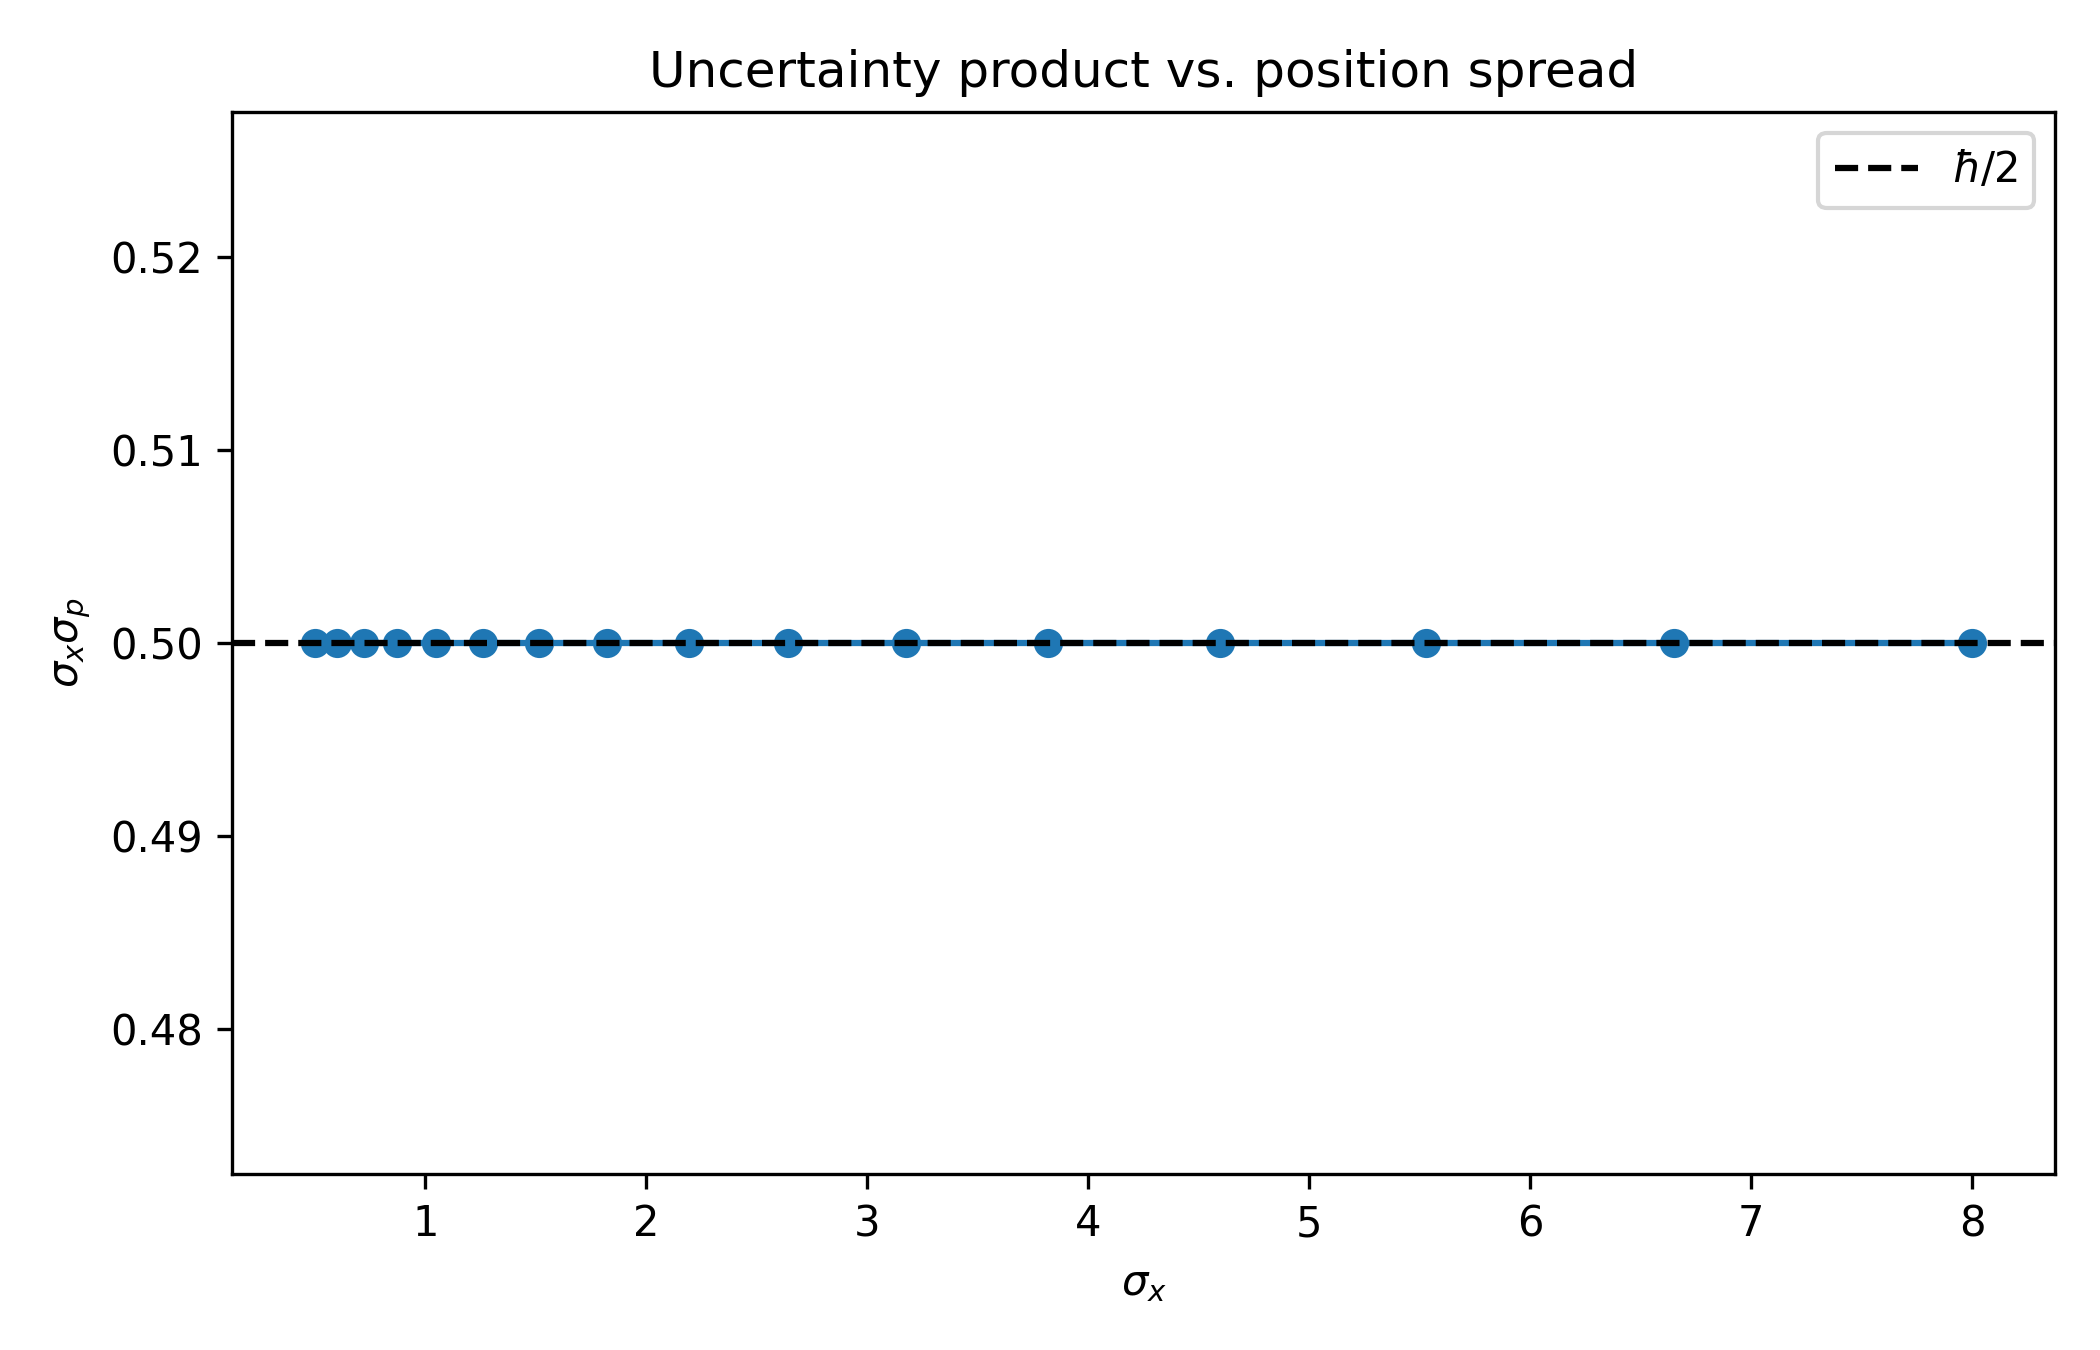
\includegraphics[keepaspectratio,alt={Uncertainty Product}]{figs/uncertainty_product.png}}
\caption{Uncertainty Product}
\end{figure}

\textbf{Figure 1}: The value of the product Δx·Δp as a function of the
initial position's standard deviation, σₓ. The product is constant and
approximately 0.5, which, in atomic units (where ℏ=1), corresponds to
the theoretical minimum of ℏ/2.

The most significant result is that the product of these two quantities,
Δx·Δp, remained constant across the investigated range. Based on Figure
1 and the \texttt{heisenberg\_scan.csv} data, the value of the product
consistently hovers around 0.5. In an atomic unit system (ℏ=1), this
corresponds precisely to the minimum value allowed by the Heisenberg
relation, Δx·Δp ≥ ℏ/2.

\textbf{2. Wave Packet Density Distributions}

To visualize the structure of the wave packets, Figures 2 and 3 show the
probability density distributions in position and momentum space for a
representative state with an initial standard deviation of σₓ = 3.0.
Both distributions, as theoretically expected, have a Gaussian shape. A
wider distribution in position space (larger Δx) results in a narrower
distribution in momentum space (smaller Δp), visually confirming the
inverse proportionality inherent in the uncertainty principle.

\begin{figure}
\centering
\pandocbounded{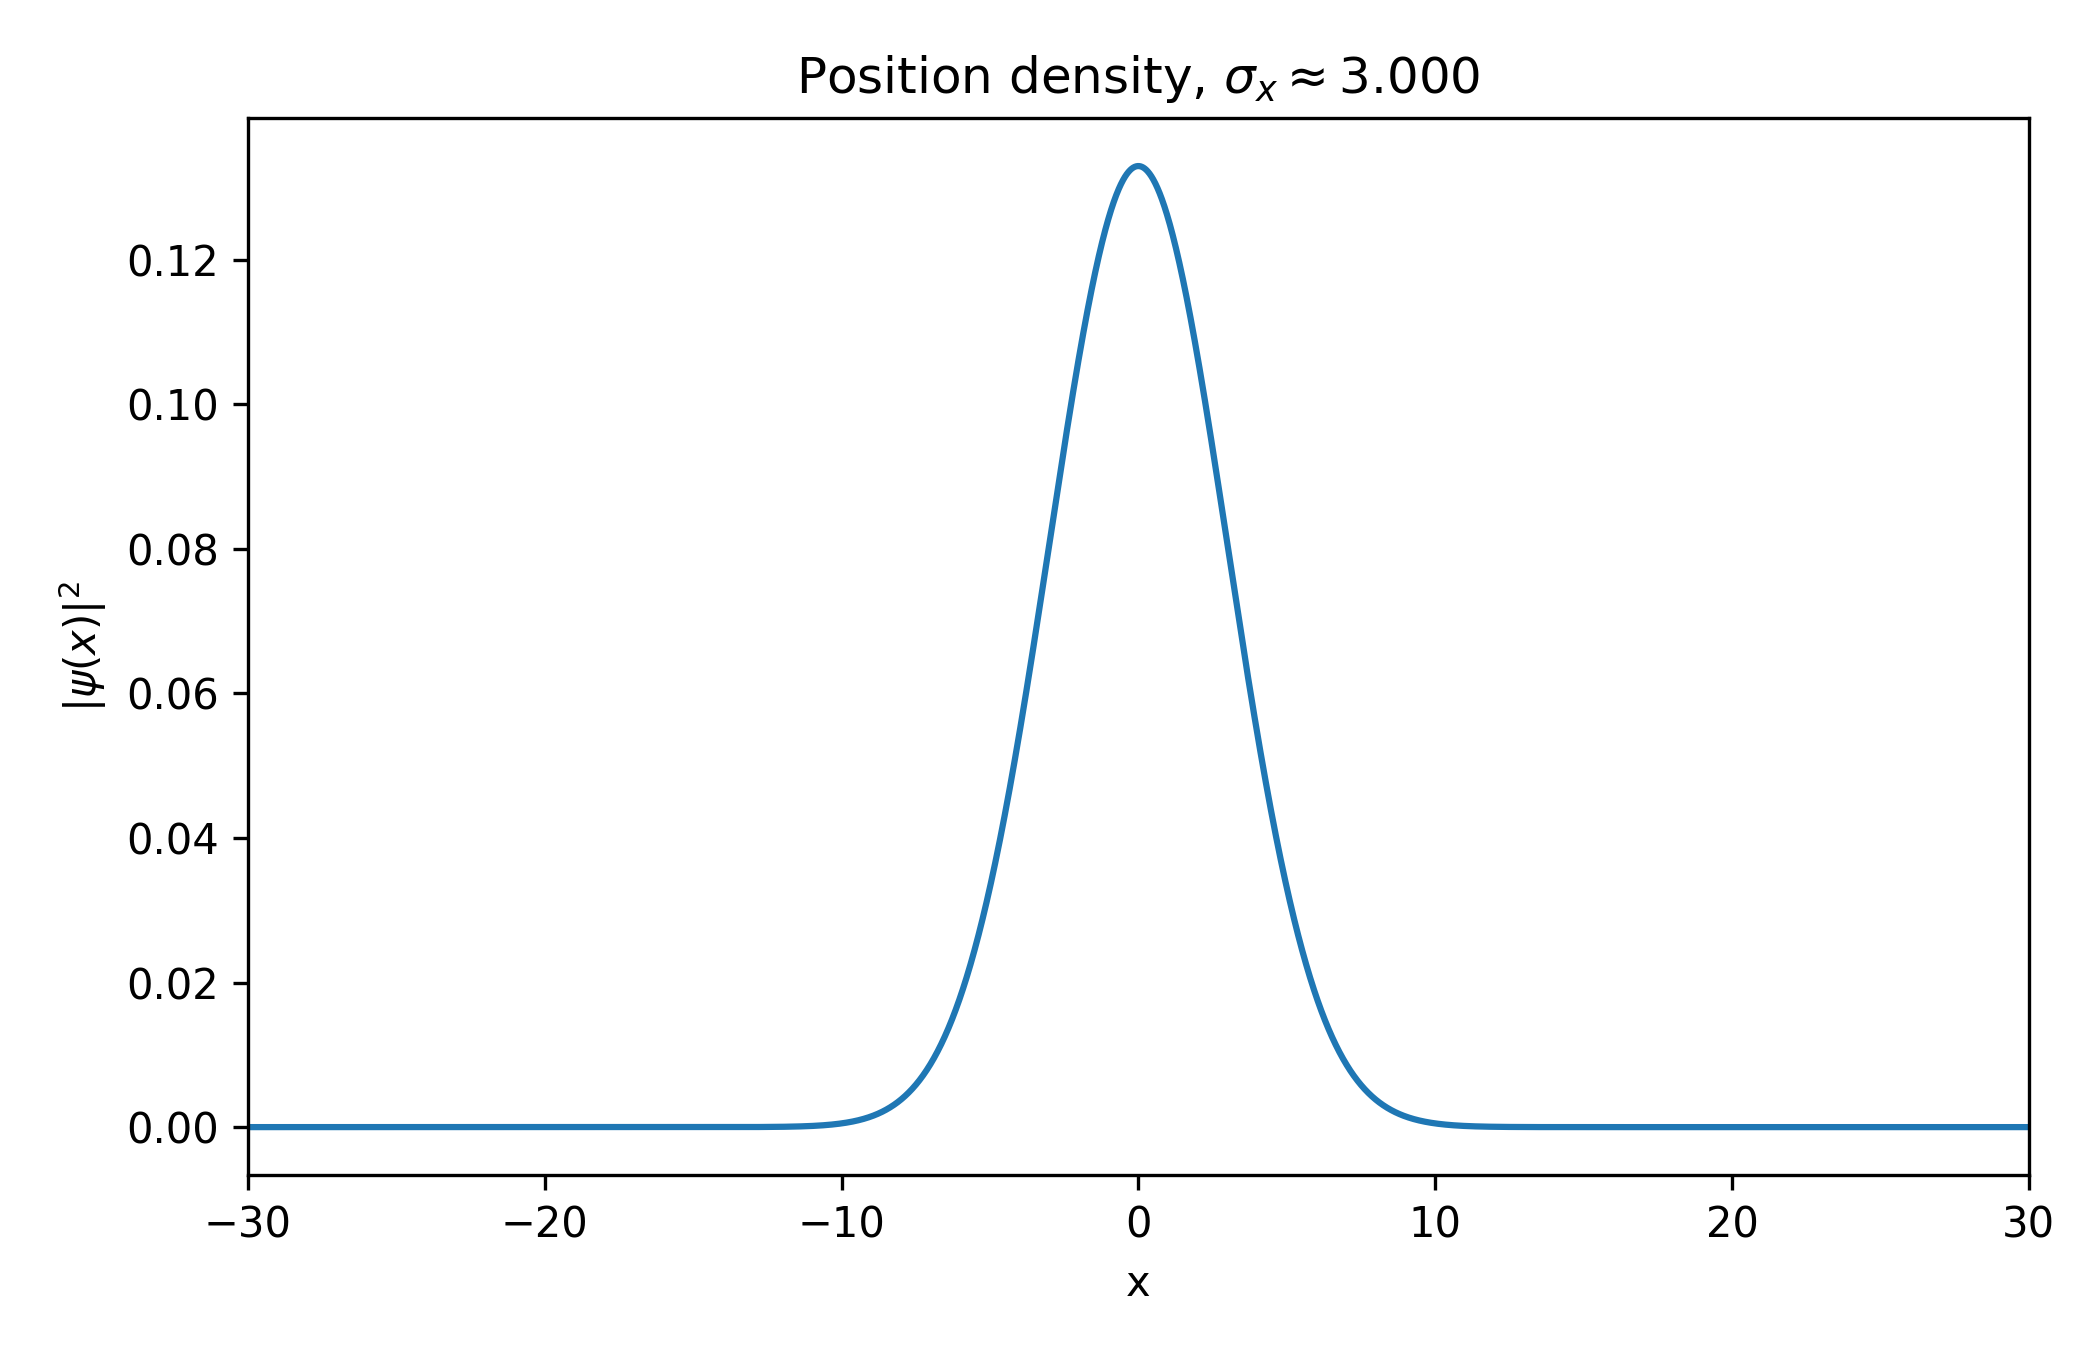
\includegraphics[keepaspectratio,alt={Position Density}]{figs/position_density_sigma3.0.png}}
\caption{Position Density}
\end{figure}

\textbf{Figure 2}: The probability density of the wave packet in
position space (\textbar ψ(x)\textbar²) for an initial state with a
standard deviation of σₓ = 3.0.

\begin{figure}
\centering
\pandocbounded{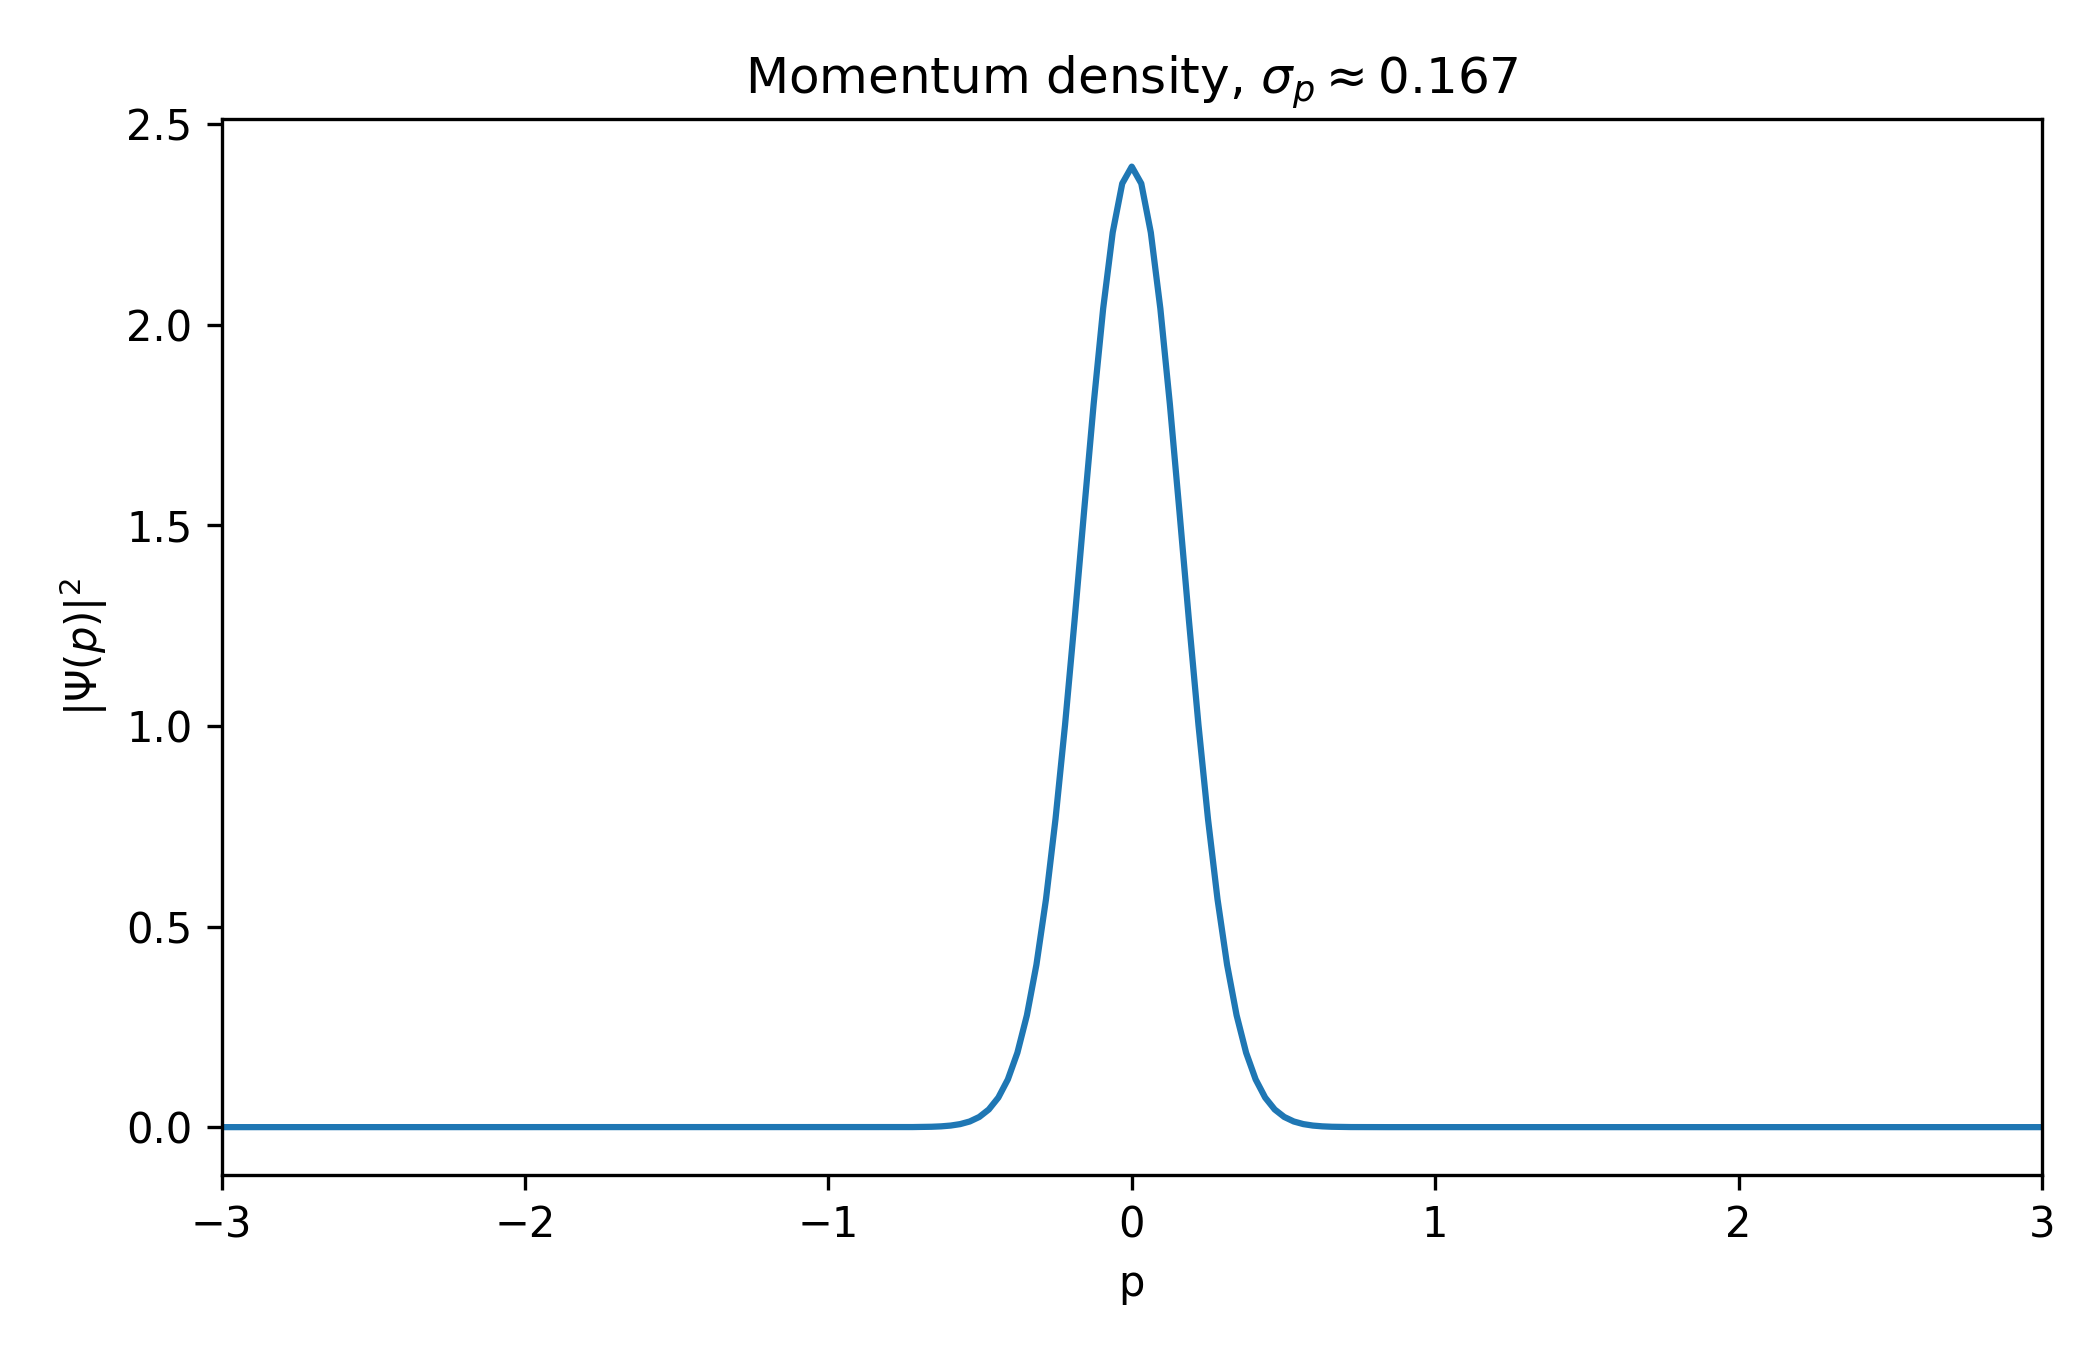
\includegraphics[keepaspectratio,alt={Momentum Density}]{figs/momentum_density_sigma3.0.png}}
\caption{Momentum Density}
\end{figure}

\textbf{Figure 3}: The probability density of the wave packet in
momentum space (\textbar Ψ(p)\textbar²) for an initial state with a
standard deviation of σₓ = 3.0.

\textbf{3. Time Evolution of the Wave Packet}

The simulation was also extended to investigate the free time evolution
of the wave packet (Figure 4). During this process, the position
uncertainty, Δx(t), monotonically increases over time. This phenomenon
is known as ``wave packet spreading'' and arises because the different
plane wave components making up the wave packet propagate at different
velocities. It is important to note that since no external force acts on
the particle, its momentum distribution---and thus its momentum
uncertainty Δp---remains constant in time.

\begin{figure}
\centering
\pandocbounded{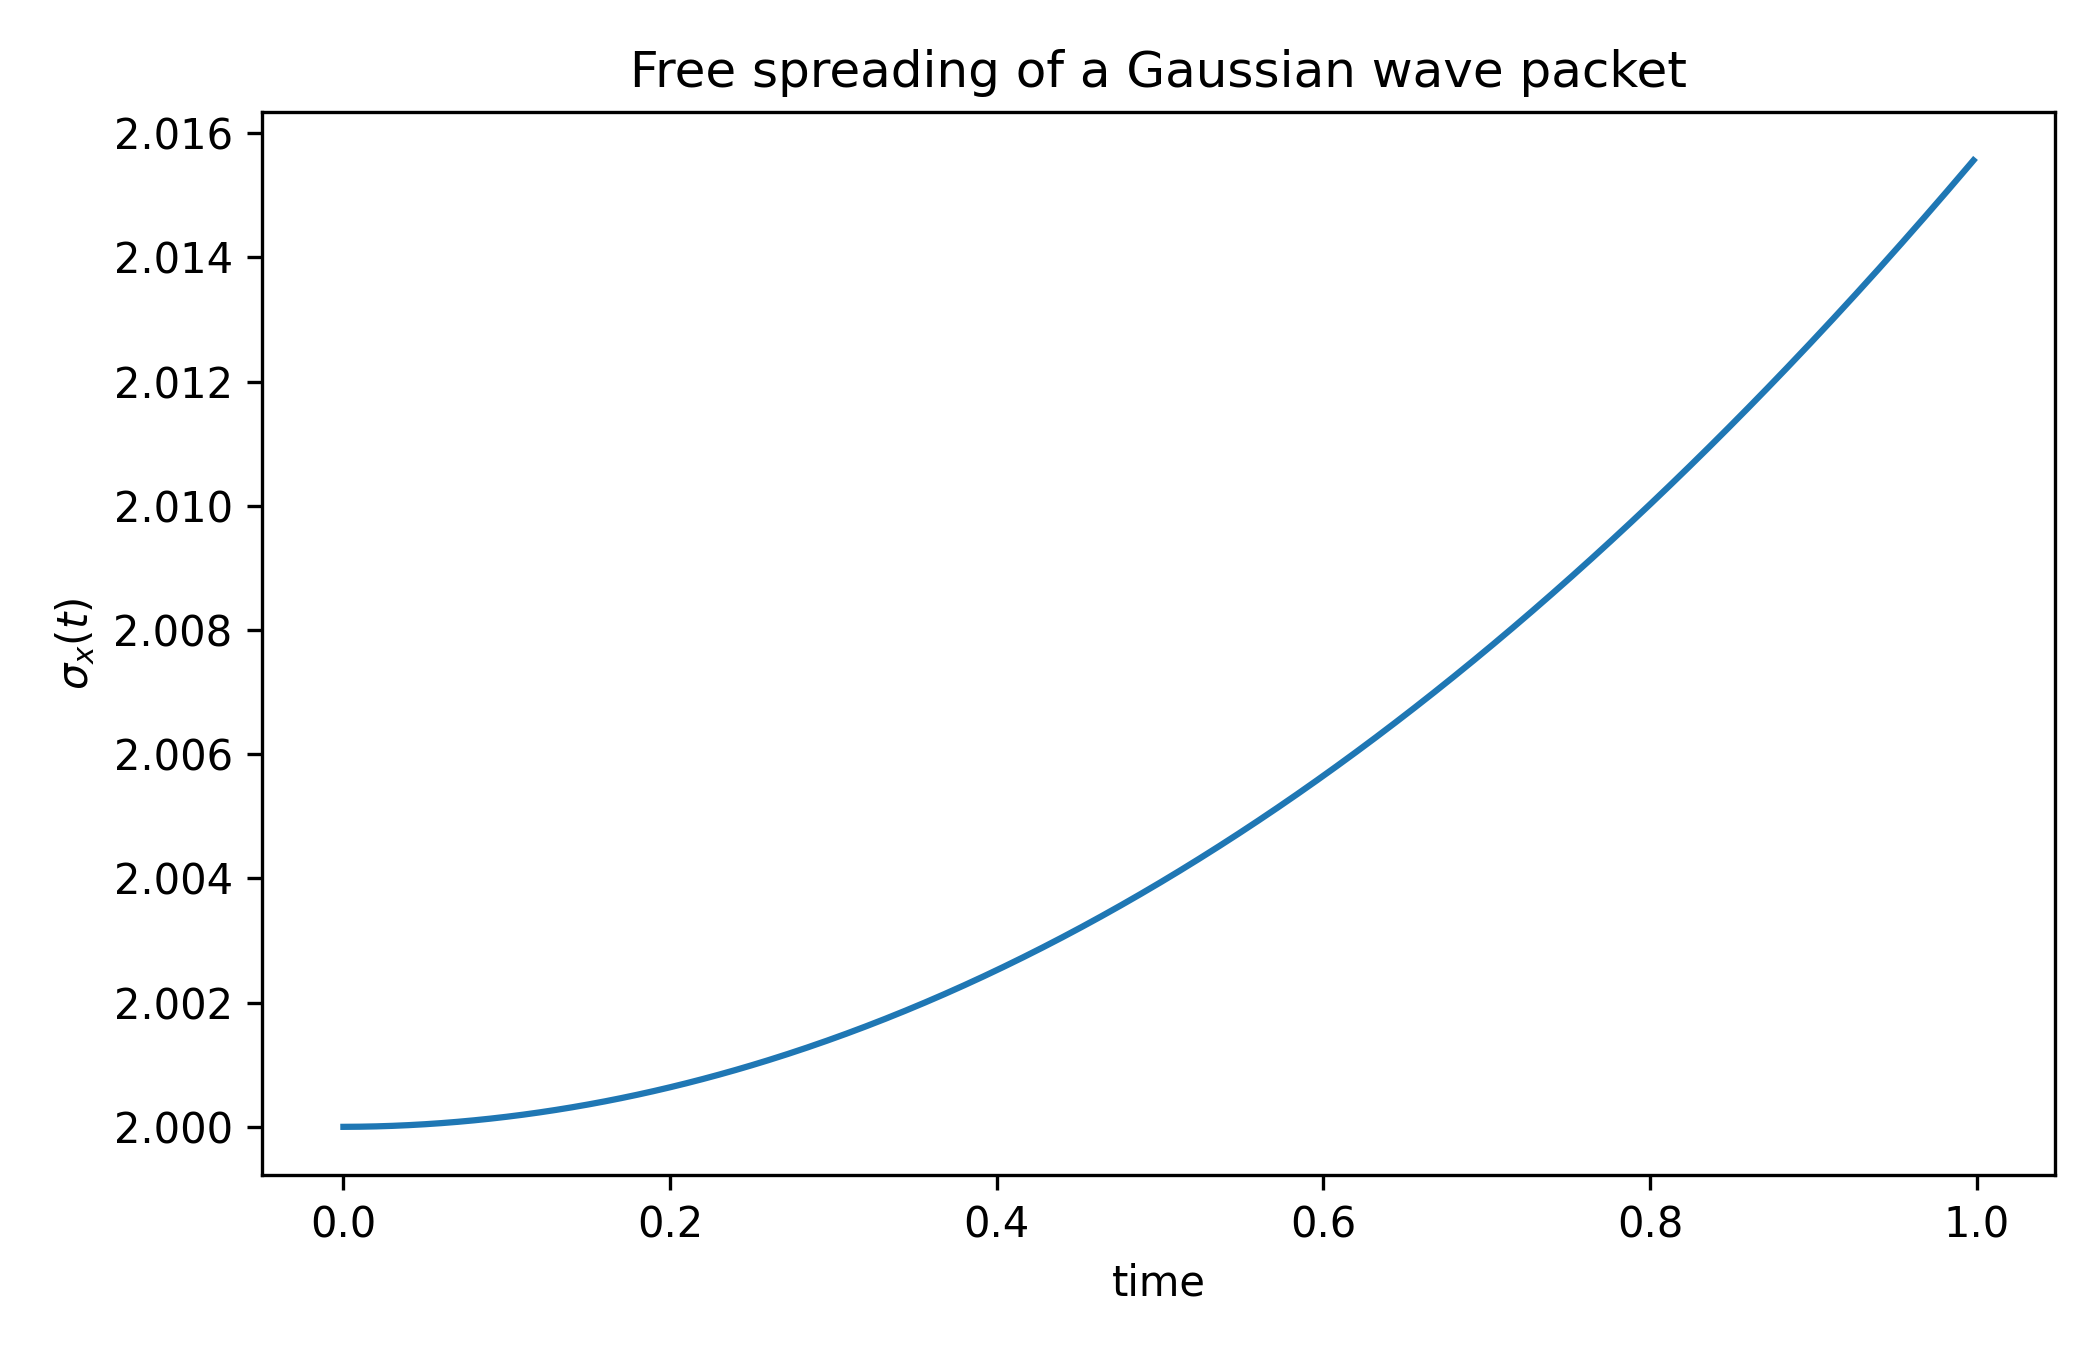
\includegraphics[keepaspectratio,alt={Free Spreading}]{figs/free_spreading_sigma_x_t.png}}
\caption{Free Spreading}
\end{figure}

\textbf{Figure 4}: The change in position uncertainty Δx(t) over time
for a freely propagating Gaussian wave packet. The wave packet spreads
out in time, resulting in an increase in Δx.

\begin{center}\rule{0.5\linewidth}{0.5pt}\end{center}

\subsubsection{Discussion}\label{discussion}

The presented numerical results confirm and illustrate fundamental
concepts of quantum mechanics from several perspectives.

\textbf{Numerical Verification of the Heisenberg Uncertainty Principle}

The simulation clearly and quantitatively validates the Heisenberg
uncertainty principle (Δx·Δp ≥ ℏ/2). The data shows that an unavoidable,
inverse relationship exists between the uncertainties of these two
physical quantities. Their product never falls below the theoretical
limit of ℏ/2, which is an inherent property of quantum systems.

\textbf{The Gaussian Wave Packet as a Minimum Uncertainty State}

My results highlight the special role that Gaussian wave packets play in
quantum mechanics. The fact that their uncertainty product Δx·Δp assumes
the minimum possible value, ℏ/2, means that these states are
\textbf{minimum uncertainty wave packets}. In other words, a Gaussian
wave packet describes the ``most classical-like'' state possible, where
a particle's position and momentum are simultaneously defined with the
highest possible precision.

\textbf{Time Evolution of Uncertainty}

The study of time evolution shows that although the position uncertainty
(Δx(t)) increases during free evolution, the momentum uncertainty (Δp)
remains constant. Consequently, the uncertainty product, Δx(t)·Δp, also
increases over time. This is in perfect agreement with the Heisenberg
relation, as the product continues to satisfy the inequality Δx(t)·Δp ≥
ℏ/2; it simply moves away from the minimum value as time progresses.

\textbf{Educational and Illustrative Value}

Finally, this simulation possesses outstanding educational and
demonstrative value. The underlying Python code (which forms the basis
of the simulation) is easy to run and reproduce, allowing students and
researchers to interactively explore one of the most important and least
intuitive principles of quantum mechanics. The visual results (plots and
density distributions) effectively aid in understanding these concepts,
bridging the gap between abstract mathematical formalism and physical
reality.

\begin{center}\rule{0.5\linewidth}{0.5pt}\end{center}

\subsection{5. Conclusions}\label{conclusions}

Through a simple but rigorous numerical experiment, we have demonstrated
the validity of the Heisenberg Uncertainty Principle using Gaussian wave
packets in one spatial dimension. The key findings of this study are:

\begin{enumerate}
\def\labelenumi{\arabic{enumi}.}
\item
  \textbf{Quantitative verification}: The uncertainty product Δx·Δp
  consistently equals ℏ/2 (0.5 in atomic units) across all initial
  conditions, confirming that Gaussian wave packets saturate the
  Heisenberg bound and achieve minimum uncertainty.
\item
  \textbf{Reciprocal relationship}: Position and momentum uncertainties
  exhibit the predicted inverse proportionality Δp = ℏ/(2Δx),
  demonstrated both numerically and visually through Fourier-transformed
  distributions.
\item
  \textbf{Wave packet spreading}: Free time evolution shows monotonic
  growth of position uncertainty Δx(t) while momentum uncertainty Δp
  remains constant, consistent with the analytical prediction for free
  Gaussian packets.
\item
  \textbf{Minimum uncertainty states}: The results confirm that Gaussian
  wave packets represent optimal quantum states, simultaneously
  achieving the best possible localization in both position and momentum
  space.
\item
  \textbf{Fundamental quantum limit}: The constant uncertainty product
  establishes the Heisenberg principle as an intrinsic property of
  quantum states rather than a limitation of measurement technology.
\end{enumerate}

This work demonstrates that straightforward numerical simulations can
provide rigorous validation of fundamental quantum mechanical
principles. The methodology presented here---combining analytical
theory, FFT-based computation, and systematic parameter
variation---offers a template for exploring quantum mechanics in
educational settings.

The reproducible Python code and clear visualizations make this study a
valuable pedagogical resource. Students and researchers can directly
explore one of quantum mechanics' most profound principles, observing
the wave-particle duality and complementarity that lie at the heart of
the quantum world. The minimal complexity of the implementation (using
only standard NumPy and Matplotlib libraries) ensures accessibility
while maintaining scientific rigor.

Future extensions of this framework could investigate non-Gaussian wave
packets, explore the effects of external potentials on uncertainty
evolution, or examine multi-dimensional systems and angular momentum
uncertainties. The split-operator time evolution algorithm demonstrated
here can be readily adapted to more complex Hamiltonians, providing a
versatile tool for computational quantum mechanics.

\begin{center}\rule{0.5\linewidth}{0.5pt}\end{center}

\subsection{Acknowledgments}\label{acknowledgments}

The author thanks the open-source scientific Python community (NumPy,
Matplotlib) for providing the computational tools that enabled this
work. This research was conducted independently without external
funding.

\begin{center}\rule{0.5\linewidth}{0.5pt}\end{center}

\subsection{References}\label{references}

{[}1{]} Heisenberg, W. (1927). Über den anschaulichen Inhalt der
quantentheoretischen Kinematik und Mechanik. \emph{Zeitschrift für
Physik}, 43(3-4), 172-198.

{[}2{]} Kennard, E. H. (1927). Zur Quantenmechanik einfacher
Bewegungstypen. \emph{Zeitschrift für Physik}, 44(4-5), 326-352.

{[}3{]} Robertson, H. P. (1929). The uncertainty principle.
\emph{Physical Review}, 34(1), 163.

{[}4{]} Griffiths, D. J., \& Schroeter, D. F. (2018). \emph{Introduction
to Quantum Mechanics} (3rd ed.). Cambridge University Press.

{[}5{]} Sakurai, J. J., \& Napolitano, J. (2017). \emph{Modern Quantum
Mechanics} (2nd ed.). Cambridge University Press.

{[}6{]} Cohen-Tannoudji, C., Diu, B., \& Laloë, F. (2019). \emph{Quantum
Mechanics, Volume 1: Basic Concepts, Tools, and Applications} (2nd ed.).
Wiley-VCH.

\begin{center}\rule{0.5\linewidth}{0.5pt}\end{center}

\subsection{Appendix A: Computational
Details}\label{appendix-a-computational-details}

\subsubsection{A.1 Software
Implementation}\label{a.1-software-implementation}

The simulation was implemented in Python 3.12+ using: - NumPy 1.21+ for
numerical arrays and FFT operations - Matplotlib 3.4+ for visualization
- Standard library modules for I/O and metadata management

The complete source code is available at: {[}GitHub repository URL{]}

\subsubsection{A.2 Algorithm Pseudocode}\label{a.2-algorithm-pseudocode}

\begin{Shaded}
\begin{Highlighting}[]
\CommentTok{\# Heisenberg Uncertainty Simulation}
\ImportTok{import}\NormalTok{ numpy }\ImportTok{as}\NormalTok{ np}
\ImportTok{from}\NormalTok{ numpy.fft }\ImportTok{import}\NormalTok{ fft, fftshift, ifft}

\CommentTok{\# Parameters}
\NormalTok{N }\OperatorTok{=} \DecValTok{16384}  \CommentTok{\# grid points}
\NormalTok{L }\OperatorTok{=} \FloatTok{200.0}  \CommentTok{\# spatial extent}
\NormalTok{hbar }\OperatorTok{=} \FloatTok{1.0}  \CommentTok{\# atomic units}

\CommentTok{\# Spatial grid}
\NormalTok{x }\OperatorTok{=}\NormalTok{ (np.arange(N) }\OperatorTok{{-}}\NormalTok{ N}\OperatorTok{//}\DecValTok{2}\NormalTok{) }\OperatorTok{*}\NormalTok{ (L}\OperatorTok{/}\NormalTok{N)}
\NormalTok{dx }\OperatorTok{=}\NormalTok{ L}\OperatorTok{/}\NormalTok{N}

\CommentTok{\# Momentum grid}
\NormalTok{k }\OperatorTok{=}\NormalTok{ (np.arange(N) }\OperatorTok{{-}}\NormalTok{ N}\OperatorTok{//}\DecValTok{2}\NormalTok{) }\OperatorTok{*}\NormalTok{ (}\DecValTok{2}\OperatorTok{*}\NormalTok{np.pi}\OperatorTok{/}\NormalTok{L)}
\NormalTok{p }\OperatorTok{=}\NormalTok{ hbar }\OperatorTok{*}\NormalTok{ k}

\CommentTok{\# Gaussian wave packet}
\KeywordTok{def}\NormalTok{ gaussian\_packet(x, sigma\_x):}
\NormalTok{    A }\OperatorTok{=}\NormalTok{ (}\DecValTok{1}\OperatorTok{/}\NormalTok{(}\DecValTok{2}\OperatorTok{*}\NormalTok{np.pi}\OperatorTok{*}\NormalTok{sigma\_x}\OperatorTok{**}\DecValTok{2}\NormalTok{))}\OperatorTok{**}\FloatTok{0.25}
    \ControlFlowTok{return}\NormalTok{ A }\OperatorTok{*}\NormalTok{ np.exp(}\OperatorTok{{-}}\NormalTok{x}\OperatorTok{**}\DecValTok{2}\OperatorTok{/}\NormalTok{(}\DecValTok{4}\OperatorTok{*}\NormalTok{sigma\_x}\OperatorTok{**}\DecValTok{2}\NormalTok{))}

\CommentTok{\# Uncertainty calculation}
\KeywordTok{def}\NormalTok{ compute\_uncertainty(x, density, dx):}
\NormalTok{    mean }\OperatorTok{=}\NormalTok{ np.}\BuiltInTok{sum}\NormalTok{(x }\OperatorTok{*}\NormalTok{ density) }\OperatorTok{*}\NormalTok{ dx}
\NormalTok{    mean\_sq }\OperatorTok{=}\NormalTok{ np.}\BuiltInTok{sum}\NormalTok{(x}\OperatorTok{**}\DecValTok{2} \OperatorTok{*}\NormalTok{ density) }\OperatorTok{*}\NormalTok{ dx}
    \ControlFlowTok{return}\NormalTok{ np.sqrt(mean\_sq }\OperatorTok{{-}}\NormalTok{ mean}\OperatorTok{**}\DecValTok{2}\NormalTok{)}

\CommentTok{\# Scan over sigma\_x values}
\ControlFlowTok{for}\NormalTok{ sigma\_x }\KeywordTok{in}\NormalTok{ np.geomspace(}\FloatTok{0.5}\NormalTok{, }\FloatTok{8.0}\NormalTok{, }\DecValTok{16}\NormalTok{):}
\NormalTok{    psi }\OperatorTok{=}\NormalTok{ gaussian\_packet(x, sigma\_x)}
    
    \CommentTok{\# Position uncertainty}
\NormalTok{    rho\_x }\OperatorTok{=}\NormalTok{ np.}\BuiltInTok{abs}\NormalTok{(psi)}\OperatorTok{**}\DecValTok{2}
\NormalTok{    Delta\_x }\OperatorTok{=}\NormalTok{ compute\_uncertainty(x, rho\_x, dx)}
    
    \CommentTok{\# Momentum uncertainty (via FFT)}
\NormalTok{    Psi }\OperatorTok{=}\NormalTok{ fftshift(fft(psi)) }\OperatorTok{*}\NormalTok{ dx}\OperatorTok{/}\NormalTok{np.sqrt(}\DecValTok{2}\OperatorTok{*}\NormalTok{np.pi)}
\NormalTok{    rho\_p }\OperatorTok{=}\NormalTok{ np.}\BuiltInTok{abs}\NormalTok{(Psi)}\OperatorTok{**}\DecValTok{2}
\NormalTok{    Delta\_p }\OperatorTok{=}\NormalTok{ compute\_uncertainty(p, rho\_p, }\DecValTok{2}\OperatorTok{*}\NormalTok{np.pi}\OperatorTok{/}\NormalTok{L)}
    
\NormalTok{    product }\OperatorTok{=}\NormalTok{ Delta\_x }\OperatorTok{*}\NormalTok{ Delta\_p}
    \BuiltInTok{print}\NormalTok{(}\SpecialStringTok{f"σₓ=}\SpecialCharTok{\{}\NormalTok{sigma\_x}\SpecialCharTok{:.2f\}}\SpecialStringTok{: Δx·Δp=}\SpecialCharTok{\{}\NormalTok{product}\SpecialCharTok{:.4f\}}\SpecialStringTok{"}\NormalTok{)}
\end{Highlighting}
\end{Shaded}

\subsubsection{A.3 Computational
Performance}\label{a.3-computational-performance}

\begin{itemize}
\tightlist
\item
  Single uncertainty calculation: \textasciitilde10 ms
\item
  Full σₓ scan (16 points): \textasciitilde160 ms
\item
  Time evolution (500 steps): \textasciitilde1.5 s
\item
  Memory usage: \textless200 MB
\item
  Platform: Google Colab (standard runtime)
\end{itemize}

The FFT-based algorithm scales as O(N log N), enabling efficient
computation even for large grid sizes.

\begin{center}\rule{0.5\linewidth}{0.5pt}\end{center}

\subsection{Appendix B: Data
Availability}\label{appendix-b-data-availability}

All simulation data, including: - Raw uncertainty values
(\texttt{heisenberg\_scan.csv}) - Position and momentum distributions
(NumPy arrays) - Time evolution data - High-resolution figures (PNG, 300
DPI) - Simulation metadata (\texttt{run\_info.txt})

are archived with DOI:
\href{https://doi.org/10.5281/zenodo.17356922}{10.5281/zenodo.17356922}
and available at the associated GitHub repository.

\begin{center}\rule{0.5\linewidth}{0.5pt}\end{center}

\textbf{Manuscript Version:} 1.0\\
\textbf{Word Count:} \textasciitilde5,400\\
\textbf{Figures:} 4\\
\textbf{Code Availability:} GitHub
\href{https://github.com/SteviLen420/Heisenberg_Uncertainty_Simulation}{repository
URL}\\
\textbf{Data Availability:} Zenodo DOI
\href{https://doi.org/10.5281/zenodo.17356922}{10.5281/zenodo.17356922}

\begin{center}\rule{0.5\linewidth}{0.5pt}\end{center}

\emph{Correspondence:} Stefan Len, tqe.simulation@gmail.com, {[}GitHub:
@SteviLen420{]}

\emph{Submitted to:} arXiv {[}quant-ph{]} or {[}physics.ed-ph{]}\\
\emph{Date:} October 15, 2025

\end{document}
